\part{Práctica 2}
\section{Actividad 2-1}
\label{p21}
\begin{center}
    \parbox{12cm}{\justify\textit{Para esta práctica, utilice el conjunto de datos de altura de ola proporcionado en Moodle.\\
    Describa las operaciones de preprocesamiento que ha realizado sobre la base de datos proporcionada y cómo queda la base de datos final ya preprocesada. Se deja a su elección el conjunto de técnicas a aplicar, así como el nivel de detalle y descripción que quiera dar a su trabajo. \\   
    Para probar rendimientos sobre su preprocesamiento, puede lanzar cualquier algoritmo de Weka, por ejemplo classifiers.functions.Logistic, y fijarse en la métrica ``Correctly Classified Instances''. En la opción ``Suplied test set'' se indicaría el fichero del conjunto de test, mientras que el de entrenamiento corresponde al que se ha cargado desde la pestaña Preprocess.}}
\end{center}

\subsection{Introducción}
En este ejercicio se van a poner en práctica los conceptos aprendidos sobre preprocesamiento de datos. Para ello se utilizará una base de datos de observaciones meteorológicas tomadas entre 2014 y 2016 a razón de 4 mediciones al día. El conjunto tiene 3559 patrones con 17 atributos numéricos y una clase nominal. Los atributos son:
\begin{itemize}
    \item AIR: Temperatura del aire en la superficie (ºK).
    \item PRES: Presión a nivel de superficie (Pa).
    \item RHUM: Humedad relativa a nivel de superficie (\%).
    \item UWND: Velocidad del viento de oeste a este (eje X) (m/s).
    \item VWND: Velocidad del viento de sur a norte (eje Y) (m/s).
    \item WDIR: Dirección del viento en el sentido de las agujas del reloj (grad).
    \item WSPD: Velocidad del viento (m/s).
    \item GST: Velocidad de pico del viento (m/s).
    \item DPD: Periodo de ola dominante (s).
    \item APD: Periodo medio de ol a dominante (s).
    \item MWD: Dirección de la que viene el periodo de ola dominante (grad).
    \item PRES: Presión a nivel de superficie (HPa).
    \item ATMP: Temperatura del aire en la parte superior de la boya (ºC).
    \item WTMP: Temperatura a nivel del mar (ºC).
    \item DEWP: Punto de rocío tomado a la misma altura que ATMP (ºC).
    \item VIS: Visibilidad desde la boya (MN).
    \item TIDE: NIvel del agua por encima o por debajo de la media inferior del agua (Pies).
\end{itemize}
La variable de salida indica la altura de ola en las seis horas siguientes. Es discreta con valores Baja, Media, Moderada y MuyAlta.

Para valorar el preprocesamiento realizado, se generará a cada paso un clasificador logístico y se evaluará con un conjunto de pruebas con la misma estructura que contiene los datos correspondientes a los años 2017 y 2018. Este proceso se realiza desde la pestaña Classify de Weka Explorer. El clasificador seleccionado será Functions.Logistic con la configuración indicada en la figura \ref{fig:classifiers-functions-logistic-config} y utilizando como conjunto de test el archivo alturaolatest.arff, al que previamente se le habrá realizado el mismo tratamiento que al conjunto de entrenamiento.

\begin{figure}[ht]
    \centering
    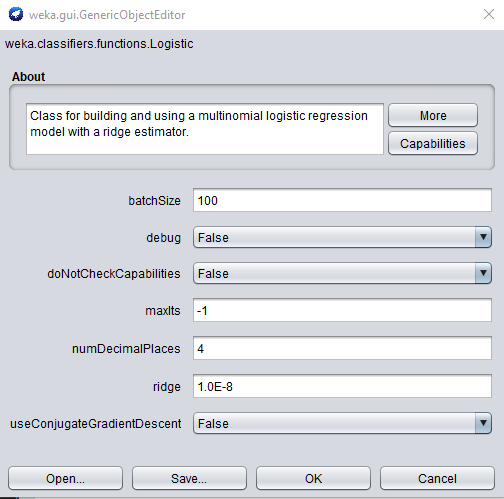
\includegraphics[scale=0.6]{classifiers-functions-logistic-config}
    \caption{Configuración del clasificador logístico}
    \label{fig:classifiers-functions-logistic-config}
\end{figure}

\subsection{Preparación}
Como paso previo se han convertido los archivos \code{.csv} a \code{.arff}. Los dos archivos se han cargado en Weka para poder visualizar su contenido, como puede verse en las figuras \ref{fig:altura-ola-orig} y \ref{fig:altura-ola-test-orig}.

\begin{figure}[H]
    \centering
    \begin{minipage}{0.5\textwidth}
        \centering
        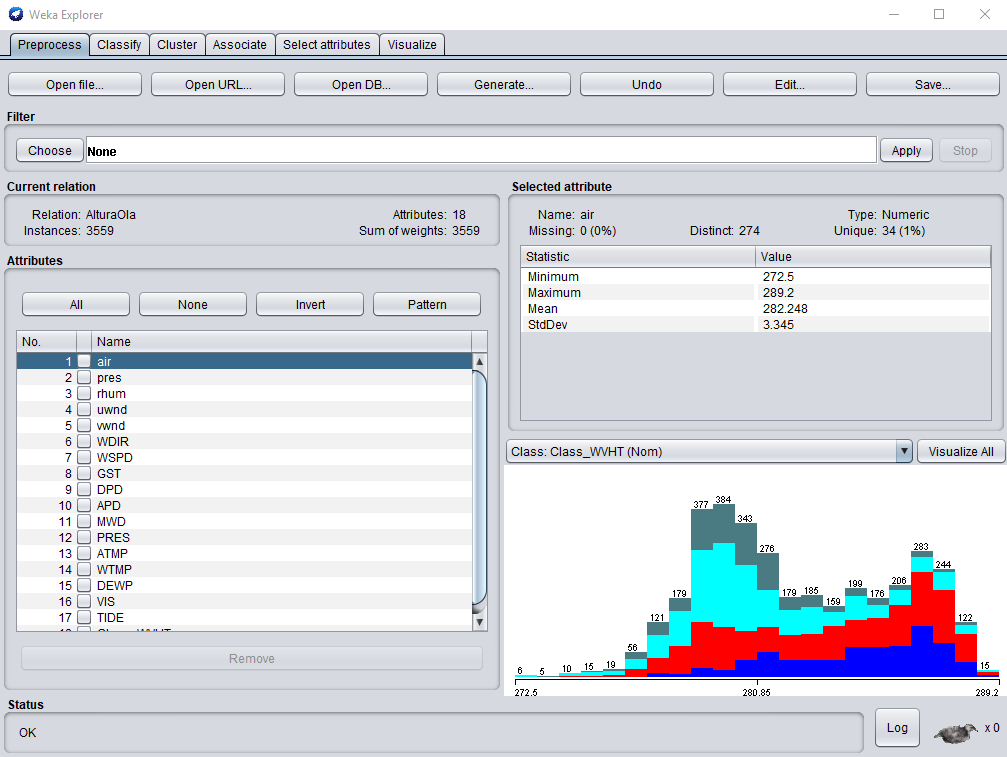
\includegraphics[scale=0.28]{altura-ola-orig}
        \caption{Captura de \code{alturaola.arff}.}
        \label{fig:altura-ola-orig}
    \end{minipage}\hfill
    \begin{minipage}{0.5\textwidth}
        \centering
        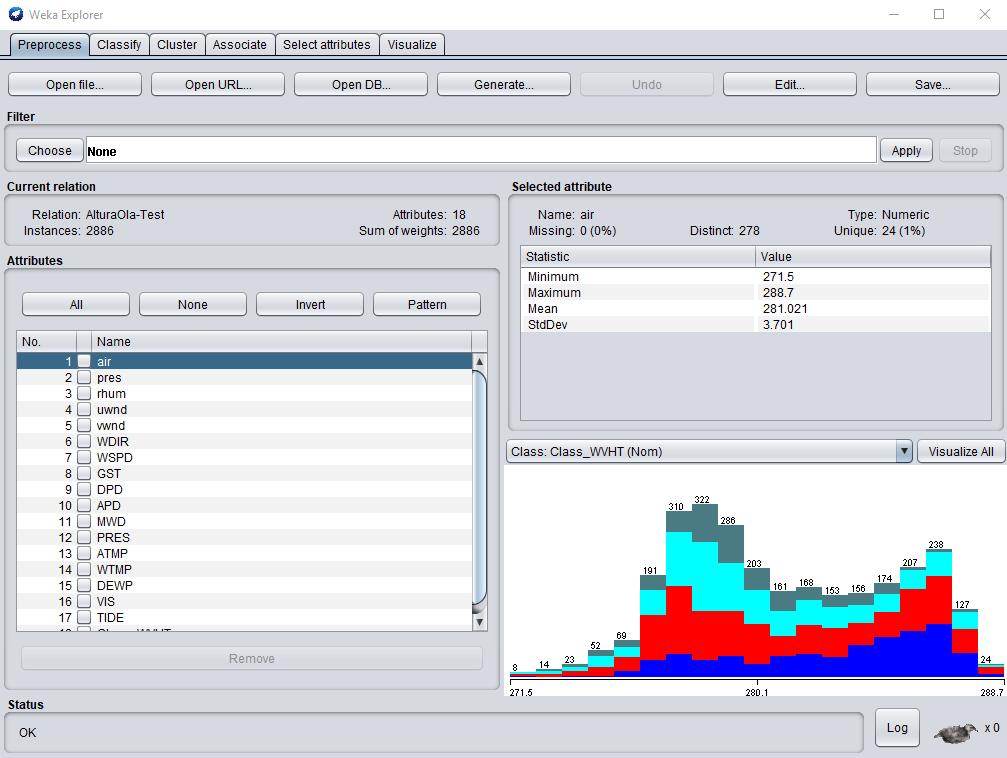
\includegraphics[scale=0.28]{altura-ola-test-orig}
        \caption{Captura de \code{alturaolatest.arff}.}
        \label{fig:altura-ola-test-orig}
    \end{minipage}
\end{figure}

Tras la conversión de los archivos y antes de empezar el tratamiento de los datos, se ha generado y testeado el clasificador logístico para ver el punto de partida. En la figura \ref{fig:clasificador-logistico-resultados-inciiales}

\begin{figure}[ht]
    \centering
    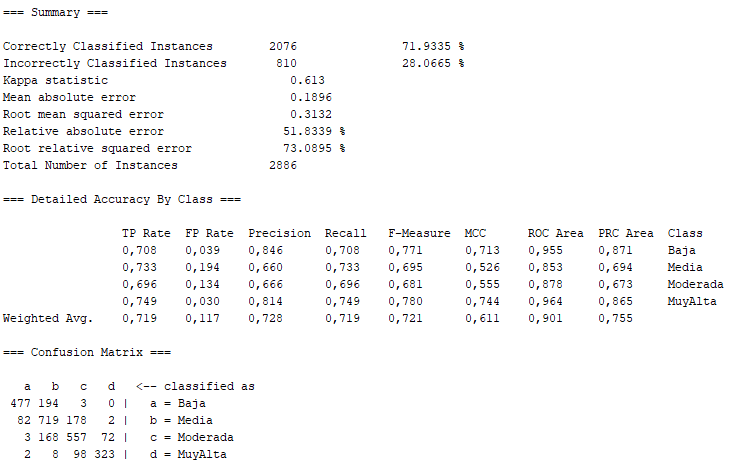
\includegraphics[scale=0.7]{clasificador-logistico-resultados-iniciales}
    \caption{Resultados del clasificador logístico antes del tratamiento de datos.}
    \label{fig:clasificador-logistico-resultados-inciiales}
\end{figure}

\subsection{Datos perdidos}
Atributos TIDS, VIS y MWD: se eliminan porque tienen 100\% de datos perdidos.
Atributo DEWP: ¿Eliminar o no?

Reemplazamiento de datos perdidos en DPD, APD, PRES y DEWP (si no se elimina).

\subsection{Unificación de medidas}
Convertir ºC a ºK
Convertir HPas a Pas

\subsection{Normalización}


\subsection{Datos extremos}


\subsection{Selección de características}

